\documentclass[12pt,a4paper]{article}
\usepackage{epsfig}
\usepackage{natbib}
\usepackage{Sweave}

%\textwidth 5in
\textheight 8in
\parskip 3mm
%\setlength{\parindent}{0mm}
\setlength{\headheight}{2 pt}

\begin{document} 

% \VignetteIndexEntry{The \texttt{ff} package: Handling Large Data Sets in R with Memory-Mapped Pages of Binary Flat Files}

\newcommand{\CPP}[1]{\emph{#1}}
\newcommand{\R}{\textbf{R}}
\newcommand{\rc}[1]{\texttt{#1}}
\newcommand{\ro}[1]{\texttt{\textsl{#1}}}



%%%%% HEADER
\begin{center}
\vspace{1.5 cm}
{\Large \textbf{The \texttt{ff} package: Handling Large Data Sets in R with Memory Mapped Pages of Binary Flat Files\\}} 
\vspace{1.0 cm} 
\textbf{\textsc{D. Adler\footnote{Corresponding author: D. Adler, email: dadler@uni-goettingen.de}, O. Nenadi{\'c}, W. Zucchini, C. Gl{\"a}ser\\}}
\vspace{0.5 cm}
\textsl{Georg-August-Universit{\"a}t G{\"o}ttingen\\ Institut f{\"u}r Statistik und {\"O}konometrie\\ Platz der G{\"o}ttinger Sieben 5\\ 37073 G{\"o}ttingen, Germany}
\end{center} 
\vspace{0.1cm} 
%%%%% END HEADER

\section{Introduction}

A current limitation of \R{} \citep{R} is that it can only address objects that fit in the available virtual memory space, currently 2-4 GB on 32-bit systems. 
Consequently the theoretical maximum length of a vector is $2^{31}$-1.
The constraints on 64-bit systems are less severe (8 GB) but still limited, and cannot cope with very large data sets \citep{Radmin}. 

The \rc{ff} package is designed to overcome this limitation. 
It extends the \R{} system by making use of a new container type in which data is stored on native binary ``flat files'' in persistent storage (hard disk, CD, DVD, etc.) rather than in the main memory.
The package enables one to work on several very large data files simultaneously.
In effect it allows one to address very large vectors or arrays which do not fit in the \R{} runtime environment. 
The idea is that one can read from and write to the flat files, and operate on the parts that have been loaded into \R{}. 
From the user's point of view the \rc{ff} objects appear to be ordinary \R{} vectors or arrays that are accessed using the usual index operators, despite the fact that the full \rc{ff} object is not resident in memory. 
The exchange of data between virtual memory and the storage device is achieved via memory mapped pages of binary files.

The \rc{ff} package comprises two layers; a low-level layer written in C++, and a high-level layer in \R{}. 
The current version of the package is 1.0 (June 30, 2007) and was prepared for the \textbf{useR! 2007} (\textit{http://www.user2007.org/}) programming competition. 
It makes use of platform-specific facilities and has been ported and tested on the following platforms: Windows, Linux, Mac OS X and FreeBSD (other BSD derivatives have not been tested but are expected to work). 
At present, support is limited to numerical data (i.e. double data type).

Section 2 describes how to get started and the usage of the package. 
It also contains examples of application involving a large data set. 
Included here is an illustration of how \rc{ff} can extend the scope of the package \rc{biglm} \citep{biglm} in that it allows one to work with even larger data sets. 
The architecture behind the \rc{ff} package is described in Section 3. 
Possible extensions of the \rc{ff} package are listed in Section 4. 


\section{Using the \texttt{ff} package}

\subsection{Getting started}

The functions \rc{ff} and \rc{ffm} are used for opening and creating flat files. 
Both functions require the argument \ro{file} that specifies the flat file. 
When the argument \ro{length} (for \rc{ff}) or \ro{dim} (for \rc{ffm}) is specified, a new flat file is created, otherwise an existing file is opened.
For example, a flat file with a length of 10 is created with

\begin{Schunk}
\begin{Sinput}
> library("ff")
> foo1 <- ff("foo1", length = 10)
> foo1
\end{Sinput}
\begin{Soutput}
$ff.attributes
   class     file pagesize readonly 
    "ff"   "foo1"  "65536"  "FALSE" 

$first.values
 [1] 0 0 0 0 0 0 0 0 0 0
\end{Soutput}
\end{Schunk}

Read and write operations on \rc{ff} objects are performed with the ``\rc{[\,]}'' and ``\rc{[\,]<-}'' operators. 
By default, the values of an \rc{ff} object are set to zero upon creation:

\begin{Schunk}
\begin{Sinput}
> foo1[1:10]
\end{Sinput}
\begin{Soutput}
 [1] 0 0 0 0 0 0 0 0 0 0
\end{Soutput}
\end{Schunk}

The entries of \rc{foo1} can be modified with the ``\rc{[\,]<-}'' operator. 
For example, the first 10 entries of the \rc{rivers} data set that contains the length of $141$ rivers in North America can be stored in an \rc{ff} object as follows:

\begin{Schunk}
\begin{Sinput}
> data("rivers")
> foo1[1:10] <- rivers[1:10]
\end{Sinput}
\end{Schunk}

At this stage it should be noted that \rc{foo1} is an \rc{ff} object while \rc{foo1[...]} returns a default R vector:
\begin{Schunk}
\begin{Sinput}
> foo1
\end{Sinput}
\begin{Soutput}
$ff.attributes
   class     file pagesize readonly 
    "ff"   "foo1"  "65536"  "FALSE" 

$first.values
 [1]  735  320  325  392  524  450 1459  135  465  600
\end{Soutput}
\begin{Sinput}
> foo1[1:10]
\end{Sinput}
\begin{Soutput}
 [1]  735  320  325  392  524  450 1459  135  465  600
\end{Soutput}
\end{Schunk}

The package provides methods for \rc{dim} and \rc{length}, e.g. the following two commands return the same value:
\begin{Schunk}
\begin{Sinput}
> length(foo1)
\end{Sinput}
\begin{Soutput}
[1] 10
\end{Soutput}
\begin{Sinput}
> length(foo1[1:10])
\end{Sinput}
\begin{Soutput}
[1] 10
\end{Soutput}
\end{Schunk}

Equivalently, sampling can be performed on the \rc{ff} object:
\begin{Schunk}
\begin{Sinput}
> set.seed(1337)
> sample(foo1, 5, replace = FALSE)
\end{Sinput}
\begin{Soutput}
[1] 735 392 524 450 600
\end{Soutput}
\end{Schunk}

The flat file object is referred to from \R{} by external pointers. In order to clear the reference, the garbage collector \rc{gc} can be used:

\begin{Schunk}
\begin{Sinput}
> rm(foo1)
> gc()
\end{Sinput}
\end{Schunk}

Calling \rc{gc()} clears the reference to the file, but it does not delete the file from the hard drive. 
Since the data is still present, the flat file can be opened again at a later stage. 
This is done with the \rc{ff} function without specifying a \ro{length} argument:

\begin{Schunk}
\begin{Sinput}
> foo1 <- ff("foo1")
> foo1
\end{Sinput}
\begin{Soutput}
$ff.attributes
   class     file pagesize readonly 
    "ff"   "foo1"  "65536"  "FALSE" 

$first.values
 [1]  735  320  325  392  524  450 1459  135  465  600
\end{Soutput}
\end{Schunk}

Note that \rc{ff} with a value for the \ro{length} argument overwrites the contents of the file.

Multi-dimensional arrays can be created with \rc{ffm}. 
For example, creating a \rc{ffm} object and storing the ``\rc{cars}'' data set (``Speed and Stopping Distances of Cars'') is performed as follows:

\begin{Schunk}
\begin{Sinput}
> foo2 <- ffm("foo2", dim = c(50, 2))
> data("cars")
> foo2[1:50, 1] <- cars[, 1]
> foo2[1:50, 2] <- cars[, 2]
\end{Sinput}
\end{Schunk}

Again, \rc{foo2} returns a \rc{ffm} object while using an index operator results in a matrix or vector being returned. 
For example, there is currently no plotting method available for \rc{ffm} objects. 
Therefore a scatterplot of the data can be created by applying the index operator:

\begin{Schunk}
\begin{Sinput}
> plot(foo2[, 1], foo2[, 2], pch = 16, las = 1)
\end{Sinput}
\end{Schunk}

Or, equivalently:

\begin{Schunk}
\begin{Sinput}
> plot(foo2[, 1:2], pch = 16, las = 1)
\end{Sinput}
\end{Schunk}
\begin{figure}[h]
  \begin{center}\fbox{
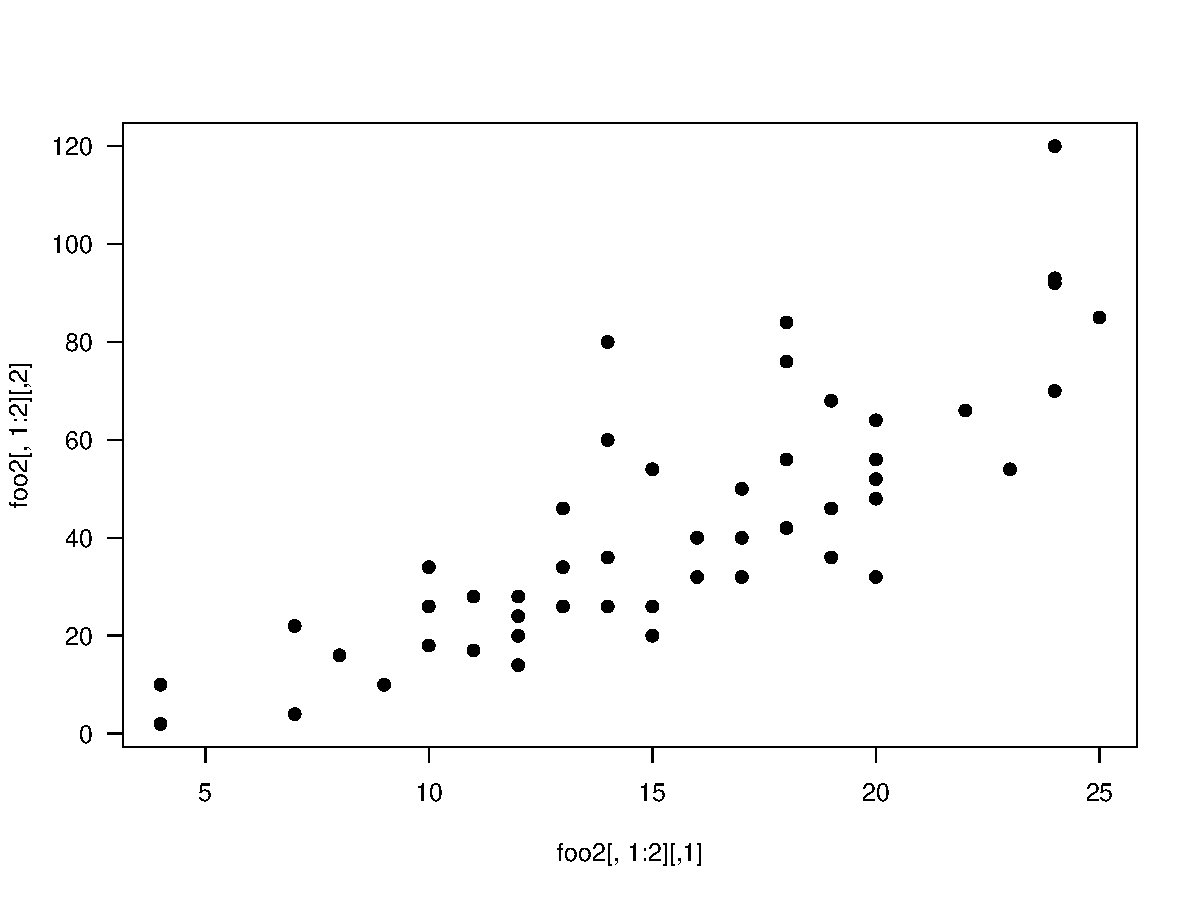
\includegraphics{figures/fig-r12}
    }
    \caption{\textsl{Scatterplot of the ``cars'' data set stored in an ff object}}
    \label{scatter0blahblahyaddablah}
  \end{center}
\end{figure}




\subsection{Examples}

For illustrating purposes we consider U.S. Census data from 2000 \citep{uscensus}. 
The data used (``Summary File 1'') contains demographic variables based on the questions asked of all people and housing units. 
The data are available from \textit{http://www2.census.gov/census\_2000/datasets/} as individual files for each of the 50 U.S. states (and the District of Columbia and Puerto Rico) as well as for the United States.

In what follows we investigate the data file for Texas based on the block level (Tables P1-P45 and P12A-P35I, c.f. U.S. Census Bureau, 2001, pp. 5-1 to 5-8). 
This data set contains records on $2465$ variables for $750624$ units. 
As a binary file (8 byte, double) the data (``P'' Tables for Texas) occupy approximately 13.7 GB. 

The data is stored in a binary flat file \textsl{texas\_p.ffd} and can be accessed via \texttt{ffm}:

%<<r13>>=
%txdata <- ffm("/tmp/texas_p")
%@
\begin{Schunk}
\begin{Sinput}
> txdata <- ffm("/tmp/texas_p")
\end{Sinput}
\end{Schunk}

In what follows the variables ``median age'' for the total, male and female population and ``average family size'' are considered. 
The variable ``median age'' is in the columns $393$-$395$ (for the total, male and female population, respectively) and the variable ``average family size'' is in column $696$. 

For the purpose of exploratory analysis it will often be of interest to examine a sample from the data rather than complete very large data sets. 
Thus, a sample of length $10000$ can be drawn from the variables mentioned above as follows:

%<<r14>>=
%# sample 10000 items
%set.seed(1337)
%ind <- runique(10000, total = 750624)
%# extract median age for males, females, both
%agb <- txdata[ind, 393]
%agm <- txdata[ind, 394]
%agf <- txdata[ind, 395]
%# extract average family size
%afs <- txdata[ind, 696]
%@
\begin{Schunk}
\begin{Sinput}
> set.seed(1337)
> ind <- runique(10000, total = 750624)
> agb <- txdata[ind, 393]
> agm <- txdata[ind, 394]
> agf <- txdata[ind, 395]
> afs <- txdata[ind, 696]
\end{Sinput}
\end{Schunk}

A simple analysis of the median ages involves the removal of missing values (which are coded as zeros here). 
A boxplot of the median ages is given in figure \ref{boxplot}.

%<<r15>>=
%## "check for complete cases"
%in.c <- agb!=0
%### remove all "0"
%agm0 <- agm[in.c]
%agf0 <- agf[in.c]
%agb0 <- agb[in.c]
%# basic summaries
%summary(agm0)
%summary(agf0)
%boxplot(agb0, agm0, agf0, names = c("total", "male", "female"), ylab = "median age", las=1)
%@
\begin{Schunk}
\begin{Sinput}
> in.c <- agb != 0
> agm0 <- agm[in.c]
> agf0 <- agf[in.c]
> agb0 <- agb[in.c]
> summary(agm0)
\end{Sinput}
\begin{Soutput}
   Min. 1st Qu.  Median    Mean 3rd Qu.    Max. 
   0.00   27.00   34.00   35.72   43.00   98.00 
\end{Soutput}
\begin{Sinput}
> summary(agf0)
\end{Sinput}
\begin{Soutput}
   Min. 1st Qu.  Median    Mean 3rd Qu.    Max. 
   0.00   29.00   37.00   38.24   46.00   96.00 
\end{Soutput}
\begin{Sinput}
> boxplot(agb0, agm0, agf0, names = c("total", "male", "female"), 
+     ylab = "median age", las = 1)
\end{Sinput}
\end{Schunk}

\begin{figure}[h]
  \begin{center}\fbox{
%<<r16, fig=TRUE, width=8, height=6, echo=FALSE>>=
%boxplot(agb0, agm0, agf0, names=c("total", "male", "female"), ylab="median age", las=1)
%@
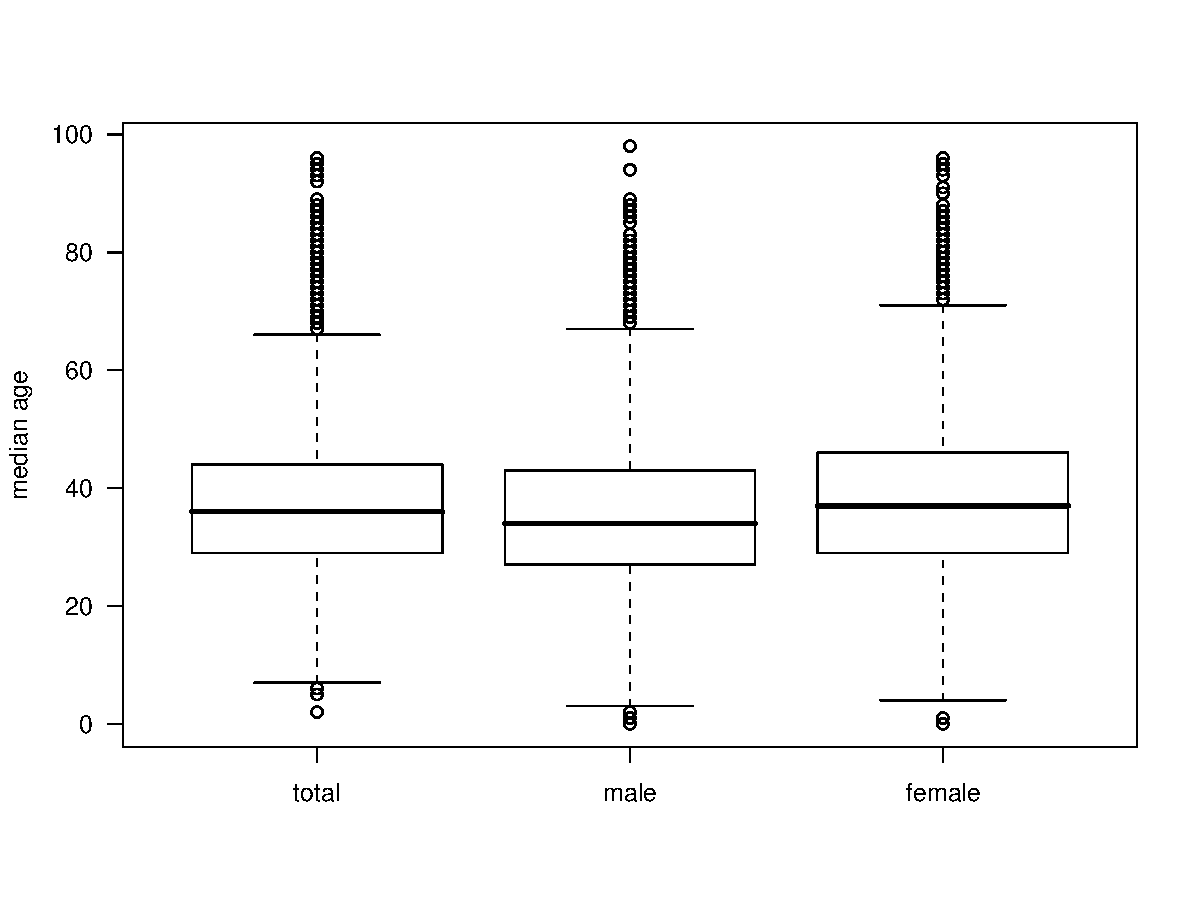
\includegraphics{figures/fig-r16}
    }
    \caption{\textsl{Boxplot for the median age (total, male and female)}}
    \label{boxplot}
  \end{center}
\end{figure}

Equivalently, one can analyse the relation between the median ages for pairwise complete cases:

%<<r17>>=
%in.c1 <- agm!=0 & agf!=0
%agb1  <- agb[in.c1]
%agm1  <- agm[in.c1]
%agf1  <- agf[in.c1]
%cor(agm1,agf1)
%@
\begin{Schunk}
\begin{Sinput}
> in.c1 <- agm != 0 & agf != 0
> agb1 <- agb[in.c1]
> agm1 <- agm[in.c1]
> agf1 <- agf[in.c1]
> cor(agm1, agf1)
\end{Sinput}
\begin{Soutput}
[1] 0.6606169
\end{Soutput}
\end{Schunk}

When drawing scatterplots of large data it is advisable to use the \rc{rgl} package \citep{rgl1,rgl2} as plotting device. 
The \rc{rgl} functions for plotting prove much more efficient for the display of large data than the default \R{} plotting device.


\begin{Sinput}
plot3d(agm1, agf1, 0, size = 4, col = "red")
view3d(0, 0, fov = 1, zoom = 0.7)
afs1 <- afs[in.c1]
afs1[afs1>10] <- 0
plot3d(agm1, agf1, afs1, size = 4, col = "red")
view3d(-60,20)
\end{Sinput}

\begin{figure}[h]
  \begin{center}\fbox{
    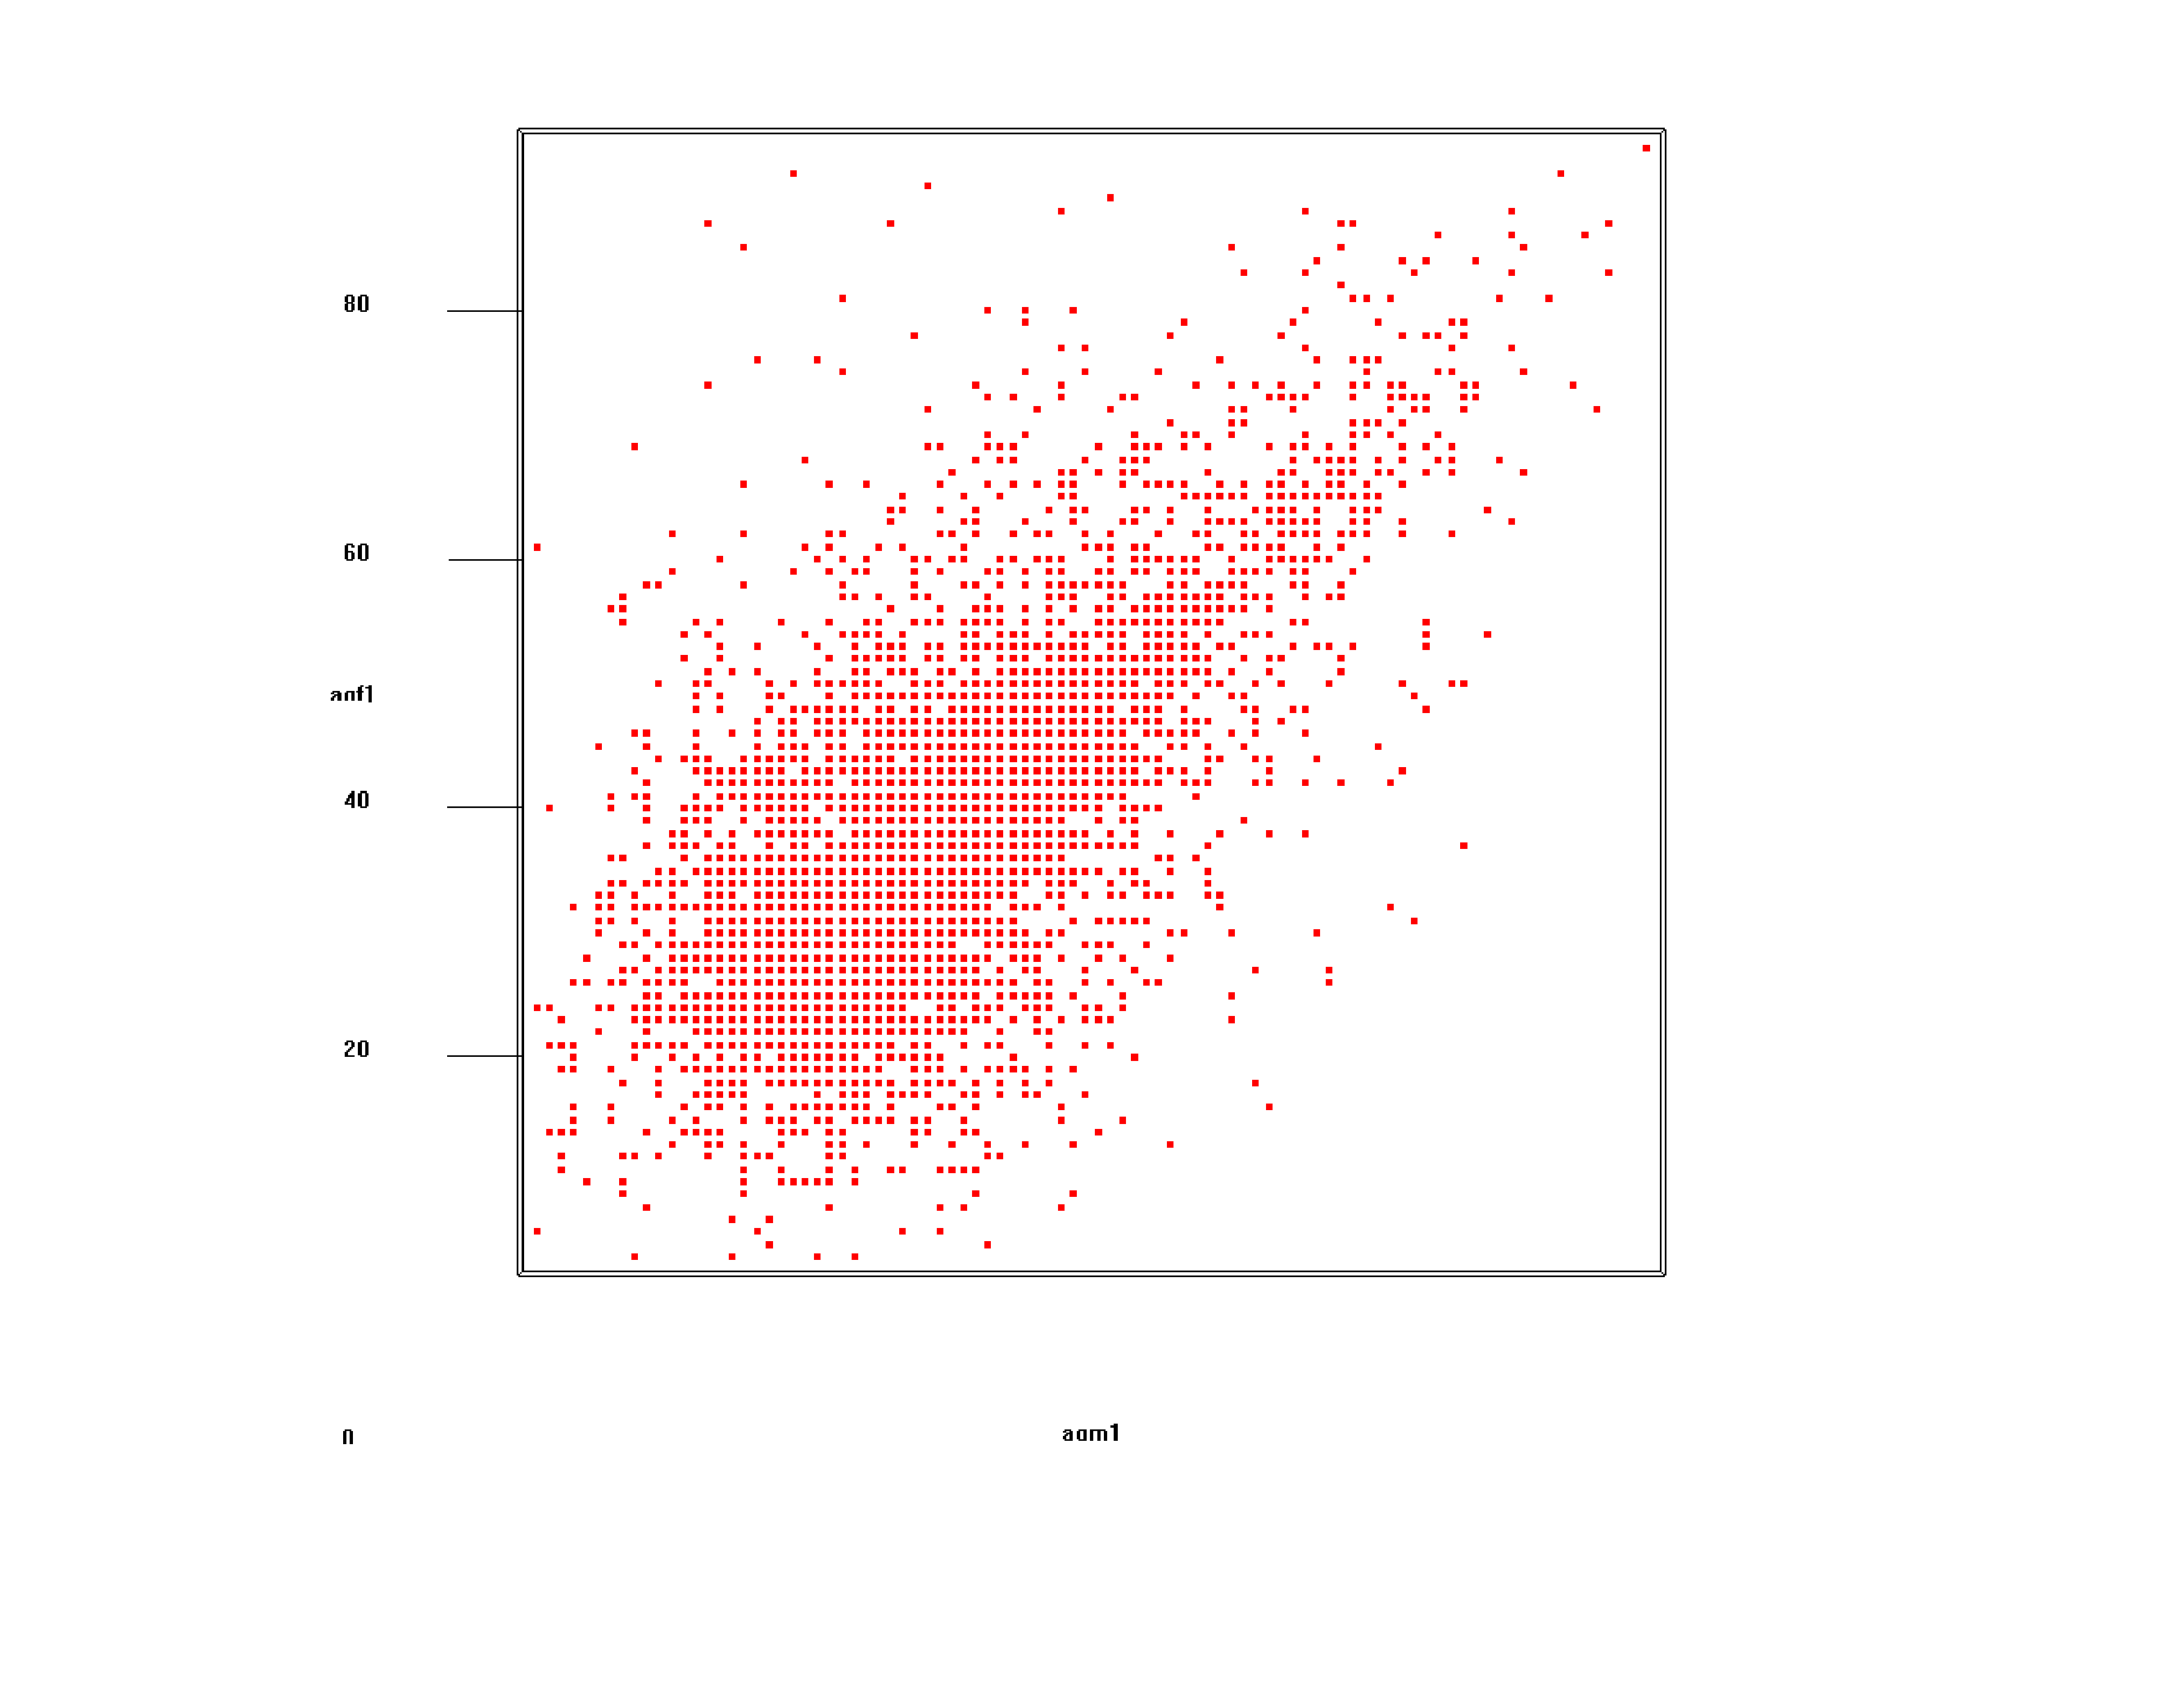
\includegraphics[width=6.5cm]{figures/rgl-001}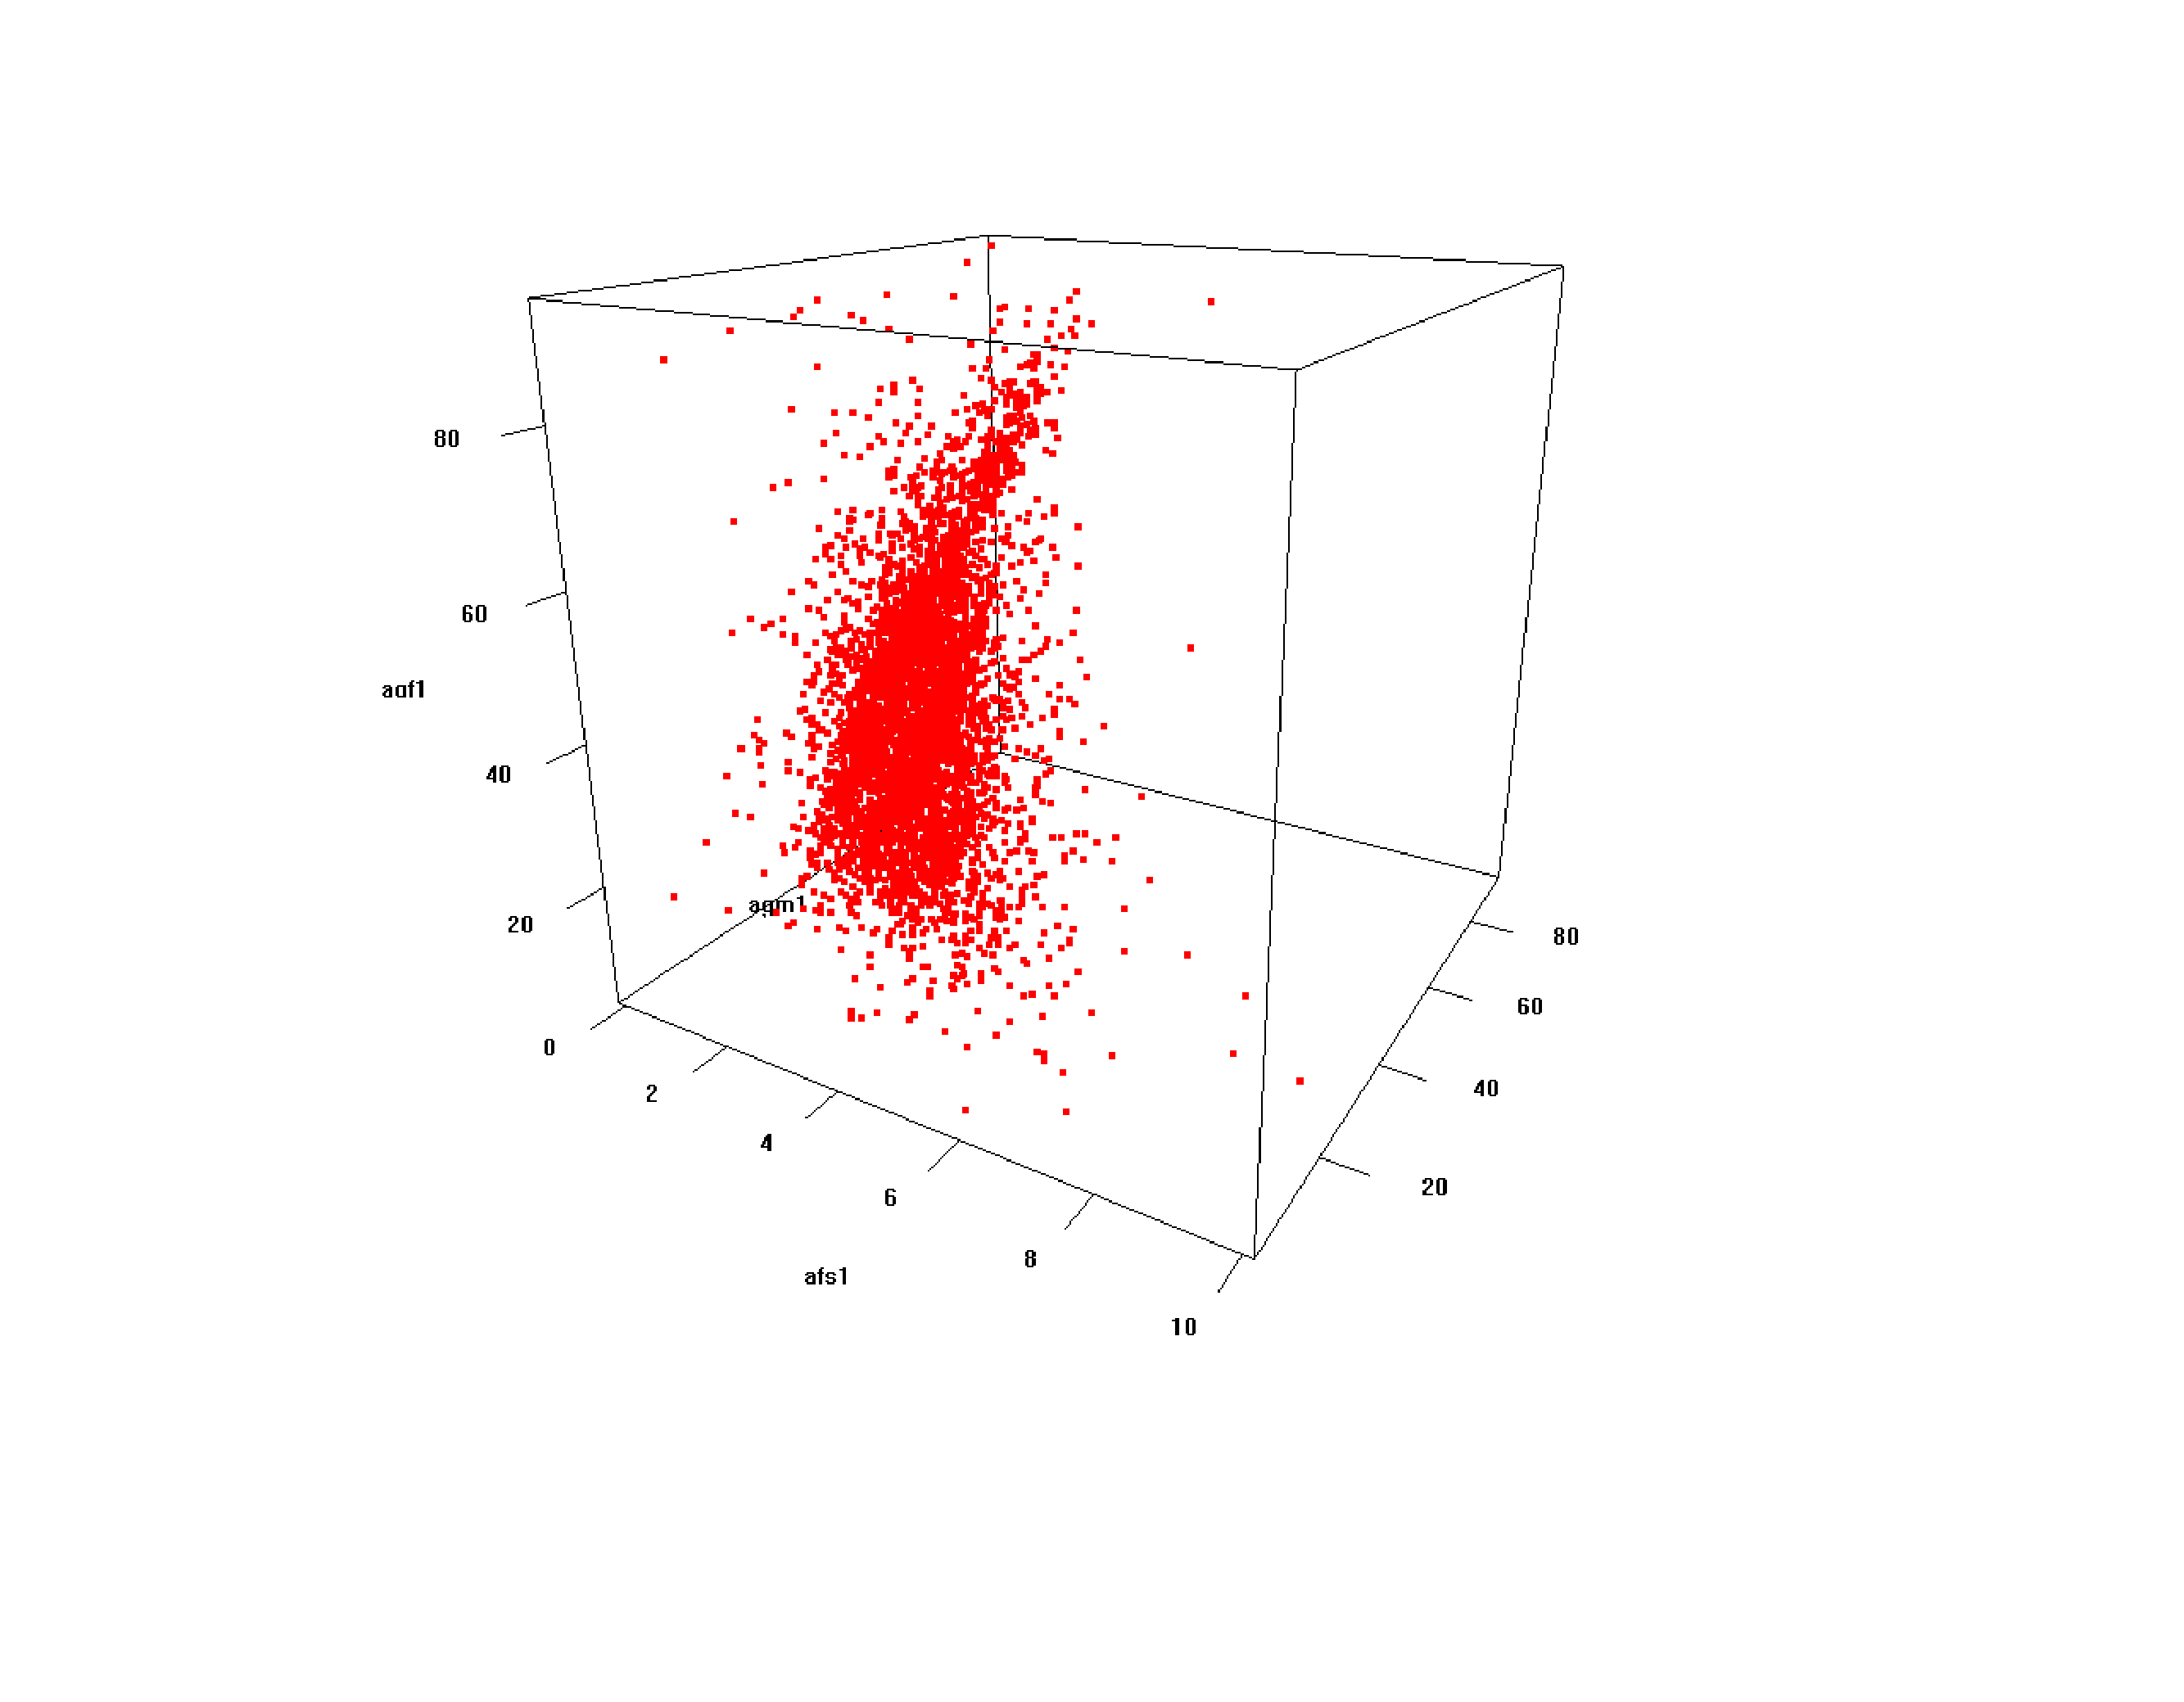
\includegraphics[width=6.5cm]{figures/rgl-002}
    }
    \caption{\textsl{Scatterplots of median age for males and females (left) and of the median age for males and females and the average family size (right)}}
    \label{scatter}
  \end{center}
\end{figure}

Figure \ref{scatter} shows two scatterplots that were created with \rc{rgl}. 
The left scatterplot in figure \ref{scatter} shows a ``2D'' view of the relation between the median age for the male and female population. 
The right scatterplot shows the relation between the median age for males and females and the average family size as a ``3D'' view.


\subsection{Interacting with the \texttt{biglm} package}

The \rc{biglm} package (``bounded memory linear regression'') provides a facility for fitting (generalized) linear models to large data sets (i.e. data sets that are larger than memory). 
By using the wrapper function \rc{ffm.data.frame} it is possible to use \rc{ffm} objects as input for the \rc{bigglm} function. 
The example provided in \rc{demo(ff.bigglm} gives a simple example on the usage. 
First, the ``\rc{trees}'' data set (``Girth, Height and Volume for Black Cherry Trees'') is converted into a \rc{ffm} object. 
After applying the wrapper function \rc{ffm.data.frame}, \rc{bigglm} can be applied equivalently to the standard case:

\begin{small}
\begin{Schunk}
\begin{Sinput}
> demo(ff.bigglm)
\end{Sinput}
\begin{Soutput}
	demo(ff.bigglm)
	---- ~~~~~~~~~

> # load 'biglm' package and 'trees' data
> require("biglm")

> data("trees")

> # create ffm object and convert 'trees' data
> m <- ffm("foom.ff", c(31, 3))

> m[1:31, 1:3] <- trees[1:31, 1:3]

> # create a ffm.data.frame wrapper around the ffm object
> ffmdf <- ffm.data.frame(m, c("Girth", "Height", "Volume"))

> # define formula and fit the model 
> fg        <- log(Volume) ~ log(Girth) + log(Height)

> trees.out <- bigglm(fg, data = trees, chunksize = 10, sandwich = TRUE)  

> ffmdf.out <- bigglm(fg, data = ffmdf, chunksize = 10, sandwich = TRUE)

> # show summaries of fitted models
> summary(trees.out)  
Large data regression model: bigglm(formula = formula, data = datafun, ...)
Sample size =  31 
              Coef   (95%    CI)    SE p
(Intercept) -6.632 -8.087 -5.176 0.728 0
log(Girth)   1.983  1.871  2.094 0.056 0
log(Height)  1.117  0.733  1.501 0.192 0
Sandwich (model-robust) standard errors

> summary(ffmdf.out)  
Large data regression model: bigglm(formula = formula, data = datafun, ...)
Sample size =  31 
              Coef   (95%    CI)    SE p
(Intercept) -6.632 -8.087 -5.176 0.728 0
log(Girth)   1.983  1.871  2.094 0.056 0
log(Height)  1.117  0.733  1.501 0.192 0
Sandwich (model-robust) standard errors

> # cleanup
> rm(m, ffmdf); invisible(gc(verbose = FALSE))
\end{Soutput}
\end{Schunk}
\end{small}


\section{Architecture}

The \rc{ff} architecture is designed around a C++ toolkit for implementing the flat file database system.
A small \R{} Application Programming Interface (API) provides transparent access to the underlying flat files using
generic interface implementations for the index-based access and mutation operators, ``\rc{[\,]}'' and ``\rc{[\,]<-}''.
Two new object classes are defined, namely \rc{ff} for vectors and \rc{ffm} for multi-dimensional arrays.   
The methods for \rc{length} and \rc{dim} operate on these two classes in the usual way.


\subsection{The C++ library}

The C++ Toolkit consists of the following parts.

\begin{itemize}
  \item Abstractions to platform-specific system services, such as memory mapped files, system pagesize queries and file system disk space usage.

  \begin{itemize}
    \item \CPP{FileMapping} class

This is a platform-specific implementation of memory mapped file facilities and exposes a factory method to create \CPP{FileSection} objects.

    \item \CPP{FileSection} class

This is a platform-specific implementation of memory mapped file regions that exposes the pointer to the virtual memory address of the file region that is mapped to main memory. 
The region can be dynamically reset to a different location of the file using a 64-bit offset, which leads to a page flush and swap.
The region size is variable in multiples of the system page size.

  \end{itemize}

\item A collection of template container classes, namely \CPP{Array<T>} and \CPP{MultiArray<T>}, which implement a caching strategy on top of memory mapped pages of large files, where \CPP{T} is the value type, e.g. \CPP{double}. 

  \begin{itemize}
    \item \CPP{Array<T>} template class

This container carries a FileMapping object and manages one \CPP{FileSection} object at a time. 
It provides a get/set method to individual cells using 64-bit indexes. 
If the requested cell is currently not served by the region provided in the \CPP{FileSection}, it is reset to the region in the file in which the cell resides. 

    \item \CPP{MultiArray<T>} template class

This container implements a multi-dimensional array using a multiple integer index.
The multi-dimensional index is translated into a one-dimensional 64-bit index that is delegated to \CPP{Array<T>}.


    \item The utility class \CPP{MultiIndex}. 

This utility class translates between multiple integer indices and a 64-bit index.
This is used to overcome the limitations of 32-bit \R{} platforms.

\end{itemize}
\end{itemize}

Figure \ref{cppt} gives an overview of the C++ toolkit and, in particular, the relationship between its components. 

\begin{figure}[h]
  \begin{center}\fbox{
    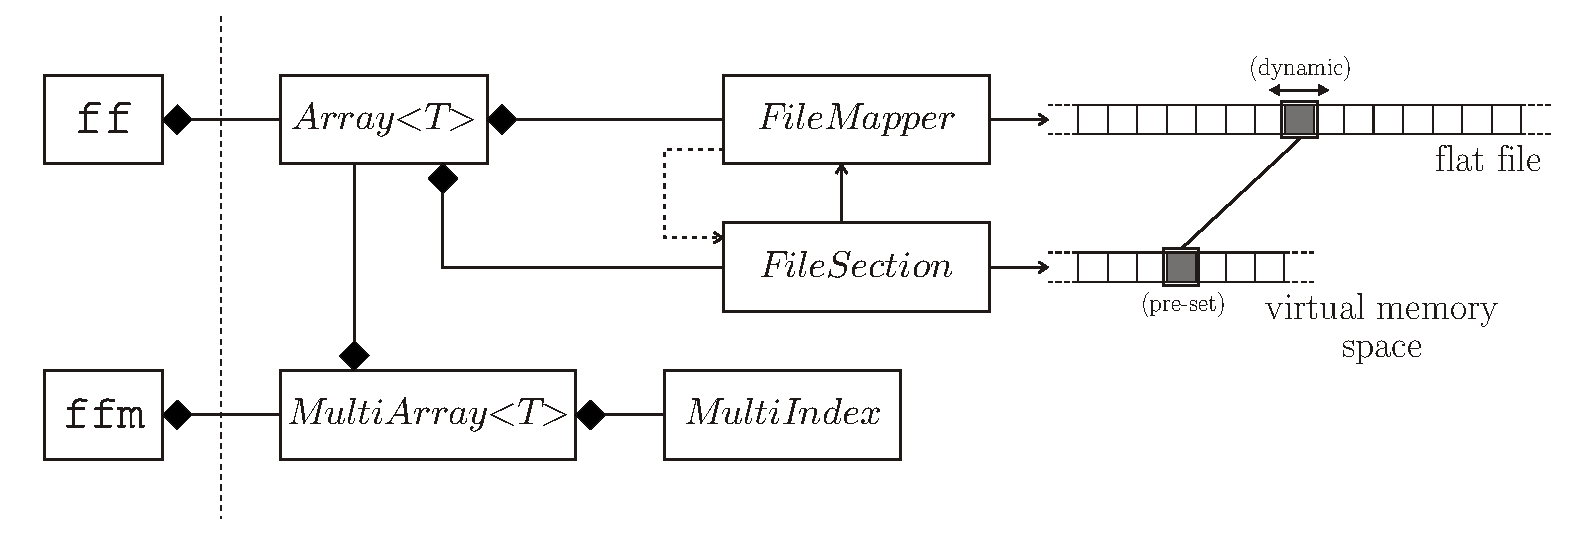
\includegraphics{figures/cpp_toolkit}
    }
    \caption{\textsl{An overview of the C++ toolkit}}
    \label{cppt}
  \end{center}
\end{figure}


The \R{} functions \rc{ff} and \rc{ffm} are essentially constructors of the C++ objects \CPP{Array<double>} and \CPP{MultiArray<double>}. 
Pointers to these objects are stored in \R{} as external pointers. 
On construction of these objects the \CPP{FileMappers} and \CPP{FileSections} are automatically created and initialized to map the first page of the file space into the virtual memory. 
On a read/write request for a particular cell the \CPP{FileSection} performs a bounding check to determine whether the requested cell is already in virtual memory. 
If it is not, the current page is flushed and the \CPP{FileSection} is mapped onto the relevant page of the file space.

In the case of \rc{ffm} the multi-dimensional index is first translated to a one-dimensional 64-bit offset; the operation then proceeds in the same way as for \rc{ff}.

The above construction is needed to overcome a limitation of \R{} integer-based indexing on 32-bit machines. 
Only 31 bits are available for an index, and consequently it is only possible to access a maximum of 16 gigabytes for an array of double-precision floating point numbers.
By using a multi-dimensional array that combines several integer indices of 31 bits, it is possible to overcome the above limitation.
The translation between multi- and one-dimensional indices is carried out in C++ because \R{} does not support 64-bit integer arithmetic.

%\underline{read/write blocks}


\subsection{The \R{} layer}

The \R{} layer contains wrapper functions and generic operators for interacting with the \CPP{Array<double>} and \CPP{MultiArray<double>} classes. 
The API comprises the following sections:
\begin{itemize}
  \item Opening / Creating  flat files
  \item I/O operations
  \item Generic functions and methods for \rc{ff} and \rc{ffm} objects
\end{itemize}

Opening and creation of flat files is controlled by the two core functions \rc{ff} and \rc{ffm}. 
When a \ro{length} (for \rc{ff}) or a \ro{dim} (for \rc{ffm}) argument is specified, a new flat file (with the corresponding size resulting from \ro{length} or \ro{dim}) is created. 
Omitting the \ro{length} or \ro{dim} argument results in loading an existing file. 
Access to flat files can be limited to read-only access in order to prevent accidental overwriting of data.

The I/O operations are controlled by the ``\rc{[\,]}'' operator (for reading) and the ``\rc{[\,]<-}'' operator (for writing). 
Methods for \rc{dim} and \rc{length} are provided for \rc{ff} and \rc{ffm} objects. 
Additionally, the function \rc{sample} is converted to a generic function and the corresponding methods for \rc{ff} and \rc{ffm} are included.

Frequent \R{} to C calls involve a calling overhead that can decrease performance when
performing I/O.
To overcome this the \rc{ff} package makes several computations on the \R{} language itself.
In the implementation of the index operator for \rc{ff} objects, the index expression gets analysed first to extract a set of sequences.
This computation is performed by the function \rc{seqpack}.
 
\begin{Schunk}
\begin{Sinput}
> library(ff)
> ind <- c(1:5, 4, 1, seq(2, 20, 4))
> seqpack(ind)
\end{Sinput}
\begin{Soutput}
     [,1] [,2] [,3] [,4]
from    1    4    1    2
to      5    4    1   18
by      1    0    0    4
\end{Soutput}
\end{Schunk}

Thus, a single \R{} to C call performs I/O on a group of sequences. 
This feature is currently only available for \rc{ff}.

When creating flat files one needs to take account of the file size limitations of the operating system's file system. 
Table \ref{fsl} gives an overview of the file size limits for selected file systems (for further details on this issue see \textit{http://en.wikipedia.org/wiki/Comparison\_of\_file\_systems}).

\begin{table}[htb]
\begin{center}
\caption{\textsl{File size limits on selected file systems}}
\label{fsl}
\begin{tabular}{ll}
  \hline\hline \textsl{File system}\hspace{3ex} & \textsl{Maximum file size} \\
  \hline
  FAT16    & 2GB \\
  FAT32    & 4GB \\
  NTFS     & 16GB \\ \hline
  ext2/3/4 & 16GB to 2TB \\
  ReiserFS & 4GB (up to version 3.4) / 8TB (from version 3.5) \\
  XFS      & 8EB (or 9EB) \\
  JFS      & 4PB \\ \hline
  HFS      & 2GB \\
  HFS Plus & 16GB \\ \hline
  USF1     & 4GB to 256TB \\
  USF2     & 512GB to 32PB \\ \hline
  UDF      & 16EB \\
\hline\hline
\end{tabular}
\end{center}
\end{table}



\section{Conclusions}

The \rc{ff} package offers the \R{} user a tool for transparently processing large data sets that don't fit into main memory using the familiar ``\rc{[\,]}'' and ``\rc{[\,]<-}'' operators. 

\R{} to C calls constitute a potential bottle-neck when performing many I/O operations from \R{}. 
The functions \rc{getrange} and \rc{seqpack} speed up these operations substantially. 
The function \rc{getrange} tests for the colon operator (``\rc{:}'') and prevents \R{} from evaluating the colon expression. 
Instead it determines the starting and ending indices and passes this information to C, thereby avoiding multiple \R{} to C calls.

A further limitation of \R{} on 32-bit platforms was also addressed, namely the 32-bit indexing limitation. 
The biggest unsigned integer, and hence the biggest index, that is directly communicable from \R{} to C is $2^{31} - 1$ which is inadequate for addressing very large data sets. 
This problem is overcome by using multi-dimensional indexing. 

The example of how the \rc{ff} package can be used in combination with \rc{biglm} illustrates the importance of chunk-based processing when dealing with very large data sets.
It is surely worthwhile to make \R{} programmers aware of this fact if they wish their functions to be applicable to very large data sets. 

\textbf{Possible extensions}

The proposed framework can be understood as a particular combination of storage policy and caching policy. 
The current implementation does not explicitly separate these components but one should regard them as separate for the purpose of future development.
The implementation in the \rc{ff} package uses memory mapped pages of files as storage policy. 
Depending on the OS-specific implementation of the memory mapping facility it might be advantageous to use I/O streaming as an alternative. 
Another alternative storage policy is to replace memory mapped pages by a connection to a database.
The latter is of interest in that it provides a natural link to databases such as MySQL.
The caching policy is single-threaded and comprises one page per unit. 
A possible alternative caching policy is to implement multiple threads for particular pre-caching strategies. 

The following features are planned in future releases: 

\begin{itemize}
  \item Currently \rc{ff} only supports the double data type. 
An obvious extension is to include other data types, such as integer, logical, float, complex, etc.  

  \item The object \rc{ffm} has not been optimized to the same extent as \rc{ff}. (This is a relatively straight-forward task.)

  \item The current implementation does not keep track of whether or not the current page has changed and therefore needs to be flushed; it always flushes. 
Ideally the OS should take care of appropriate flushing behaviour. 
Nevertheless it is worth checking whether or not this is the case, to avoid unnecessary flushing. 

  \item Currently the size of the flat files is fixed. It might be useful to have \rc{append} and \rc{truncate} functions. 

\end{itemize}

Of course future extensions will also depend on feedback and requests from users.



%%%%% REFERENCES
%\section{References}
\bibliographystyle{agsm}
\bibliography{_lit}


\end{document}
